\documentclass[11pt,a4paper]{article}
\usepackage[margin=19mm]{geometry}
\usepackage[T1]{fontenc}\usepackage{tgheros,textcomp}
\renewcommand{\familydefault}{\sfdefault}
\usepackage{xcolor,tikz,hyperref}
\usetikzlibrary{arrows.meta,calc}
\definecolor{navy}{HTML}{171717}\definecolor{teal}{HTML}{242424}
\definecolor{gold}{HTML}{A0A0A0}\definecolor{pale}{HTML}{F2F2F2}
\definecolor{muted}{HTML}{626262}
\hypersetup{colorlinks=true,urlcolor=teal,pdftitle={Aktina executive summary},pdfauthor={Loukas Louka; Aktina team}}
\pagestyle{empty}\setlength{\parindent}{0pt}\setlength{\parskip}{7pt}
\color{navy}
\begin{document}
{\small\color{teal} AKTINA \hfill PAFOS 2.0 / TEAM REVIEW DRAFT}
\vspace{12mm}

{\fontsize{35}{39}\selectfont\bfseries Make water with\par surplus solar.}

\vspace{3mm}
{\large Cyprus curtails solar generation while water production needs electricity.\par Make drinking water during that window; store it for Paphos's later demand.}

\vspace{8mm}
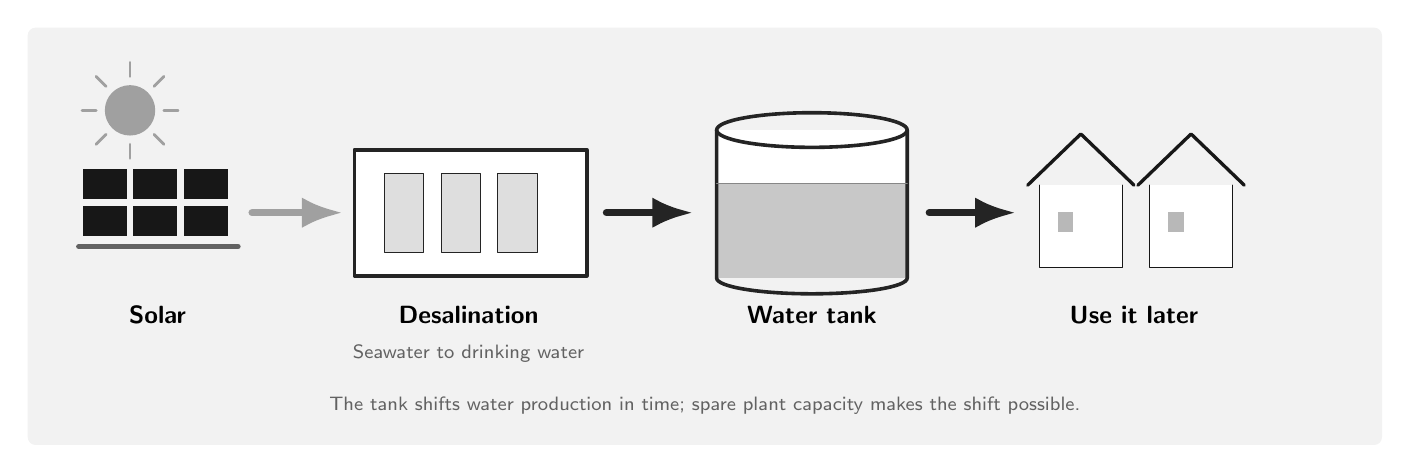
\begin{tikzpicture}[x=1cm,y=1cm,>=Latex,line cap=round,line join=round]
\fill[pale,rounded corners=1mm] (0,0) rectangle (17.2,5.3);
\fill[gold] (1.3,4.25) circle (.32);
\foreach \a in {0,45,...,315}{\draw[gold,line width=1pt] (1.3,4.25) ++(\a:.43)--++(\a:.18);}
\foreach \i in {0,1,2}{\foreach \j in {0,1}{\fill[navy] (0.7+\i*.64,2.65+\j*.47) rectangle ++(.56,.38);}}
\draw[muted,line width=2pt] (.65,2.52)--(2.67,2.52);
\node[font=\bfseries\small] at (1.65,1.65) {Solar};
\draw[gold,line width=2.6pt,->] (2.85,2.95)--(4.0,2.95);
\fill[white,rounded corners=0mm] (4.15,2.15) rectangle (7.1,3.75);
\draw[teal,line width=1.3pt,rounded corners=0mm] (4.15,2.15) rectangle (7.1,3.75);
\foreach \i in {0,1,2}{\fill[teal!15] (4.53+\i*.72,2.45) rectangle ++(.5,1.0);\draw[teal] (4.53+\i*.72,2.45) rectangle ++(.5,1.0);}
\node[font=\bfseries\small] at (5.6,1.65) {Desalination};
\node[font=\scriptsize,text=muted] at (5.6,1.16) {Seawater to drinking water};
\draw[teal,line width=2.6pt,->] (7.35,2.95)--(8.45,2.95);
\fill[white] (8.75,2.12) rectangle (11.17,4.0);
\fill[teal!25] (8.75,2.12) rectangle (11.17,3.32);
\draw[teal,line width=1.3pt] (8.75,4)--(8.75,2.12) arc[start angle=180,end angle=360,x radius=1.21,y radius=.2]--(11.17,4);
\draw[teal,line width=1.3pt] (9.96,4) ellipse (1.21 and .22);
\draw[teal!55] (8.75,3.32)--(11.17,3.32);
\node[font=\bfseries\small] at (9.96,1.65) {Water tank};
\draw[teal,line width=2.6pt,->] (11.45,2.95)--(12.55,2.95);
\foreach \i in {0,1}{\fill[white] (12.85+\i*1.4,2.25) rectangle ++(1.05,1.05);\draw[navy,line width=1.2pt] (12.7+\i*1.4,3.3)--++(.675,.65)--++(.675,-.65);\draw[navy] (12.85+\i*1.4,3.3)--++(0,-1.05)--++(1.05,0)--++(0,1.05);\fill[gold!75] (13.08+\i*1.4,2.7) rectangle ++(.2,.26);}
\node[font=\bfseries\small] at (14.05,1.65) {Use it later};
\node[font=\scriptsize,text=muted] at (8.6,.5) {The tank shifts water production in time; spare plant capacity makes the shift possible.};
\end{tikzpicture}

\vspace{6mm}
\begin{minipage}[t]{.48\linewidth}
{\large\bfseries What we have}\par
A local demo with 296 supplied days: sun, production, tank level and illustrative cost. On 3 July, supplied production costs \texteuro2,628 versus \texteuro2,995 for flat production, with equal daily water and ending stock.

The supplied schedule uses persistence. Stefanos's LightGBM forecasts are shown separately. The intended final schedule awaits his confirmation.
\end{minipage}\hfill
\begin{minipage}[t]{.47\linewidth}
{\large\bfseries What we need}\par
The original test favours persistence. Archived weather forecasts improve retrospective F1 to 98.41\%; residual corrections reduce MAE further but add one false alarm. No learned correction is promoted; live performance is unproven.

A pilot needs operator limits, demand, tariffs and curtailment signals. Recovered solar and field savings remain unmeasured. Grid and the separate Sites prototype retain untested business models.
\end{minipage}

\vfill
\hrule height .5pt\vspace{3mm}
{\footnotesize Concept, application and evaluation: Loukas Louka. Original model, scheduler and roadmap: Stefanos. Business: Andreas Nikolaides and Cleopas Cleopa.\par
Evidence: \href{https://github.com/stefanosbordea/actina/tree/stefanos-model/app/handoff}{retained handoff and schedule reproduction}; \href{https://aktina-pafos-2026.vercel.app/benchmark.html}{AktinaBench}. Historical weather, illustrative plant and prices; no plant connection. Updated 4 October 2026.}
\end{document}
